\section{In-Context-Learning of Black-Scholes}

As an extension of the work presented in \cite{garg2022what}, we intent to test the learning-to-learn and predictive abilities of transformer on a real world financial application: the European Option Market. 

\subsection{Introduction to Black-Scholes}

Relevant financial glossary is defined in \ref{app:glossary}.

Consider a stock that trades at \emph{spot price} $S$ today. A \emph{call option} on this stock
gives its holder the right, but not the obligation, to buy the stock at a fixed
\emph{strike} price $K$ at a fixed \emph{maturity} $T$ years from now.
This call option has a price $C$ today, which is usually much smaller than the stock price, and depends strongly on how much the stock's \emph{volatility} $\sigma$. A worked example is presented in appendix \ref{app:call_price}.


Price $S$, strike $K$ and maturity $T$ and are written in the contract and observable, but the volatility $\sigma$ is not. In practice it is inferred from the prices of other options
on the same stock. This is precisely an in-context
learning problem: given example (option, price) pairs on one stock, predict the price of
another option on that stock.

The Black-Scholes model makes this relationship precise. We define a new family of
functions, Black-Scholes functions, as
\begin{equation}
  \frac{C}{S} = \Phi(d_1) - e^{m - rT}\,\Phi(d_2), \qquad
  d_1 = \frac{-m + \left(r + \tfrac{1}{2}\sigma^2\right)T}{\sigma\sqrt{T}}, \qquad
  d_2 = d_1 - \sigma\sqrt{T},
  \label{bs}
\end{equation}
with $C, S, K, T$ as previously, $m = \ln(K/S)$ is the log-moneyness, $r = 0.02$ the risk-free rate (known), and $\Phi$ the standard normal CDF.
The function is non-linear but low dimensional: two inputs/features $(m, T)$ and one unknown parameters $\sigma$.

The unknown volatility $\sigma$ should be learned by the transformer from in-context
examples, and used to infer the standardised call price $C/S$ of a new option on the same asset.
We consider two variations of the problem: (i) \emph{flat volatility}, each
prompt has a constant volatility sampled  $\sigma \sim U[0.1, 0.5]$ per prompt. (ii)
\emph{smile volatility},
\begin{equation}
  \sigma(m) = \max\{\sigma_0 + b\,m + c\,m^2,\ 0.05\}, \quad
  \sigma_0 \sim U[0.15, 0.4],\ b \sim U[-0.4, 0],\ c \sim U[0, 1].
\end{equation}
The latter takes into account that implied volatility observed in markets varies with strike (skew $b$ and curvature $c$), and is therefore a more
realistic model. Consequently the transformer must effectively infer three parameters from the context instead of one, as in the flat volatility setting.

\subsection{Training and evaluation setup}

We use the same training setup as described in \cite{garg2022what}, except that the
curriculum only increases the number of examples, since $d = 2$ is fixed. The prompt is
\begin{equation}
P_{BS} = \big(x_1, f_\theta(x_1), \dots, x_k, f_\theta(x_k), x_{\text{query}}\big),
\qquad x_i, x_{\text{query}} \sim \mathcal{N}(0, I_2),
\end{equation}
where the hidden volatility parameters $\theta$, $\sigma$ for flat and $(\sigma_0, b, c)$
for smile volatility, are drawn once per prompt. As in \cite{garg2022what}, the inputs are
Gaussian; they are mapped to option features $m(x)$ and $T(x)$ by
Table~\ref{tab:bs-inputs}.

\begin{table}[h]
\caption{Input encoding for the Black--Scholes tasks ($d = 2$).}
\label{tab:bs-inputs}
\centering
\small
\begin{tabular}{lll}
\toprule
Input & Option feature & Meaning \\
\midrule
$x^{(1)}$ & log-moneyness $m = 0.2\,x^{(1)}$
  & strike relative to today's price, $m = \ln(K/S)$ \\
$x^{(2)}$ & maturity $T = 0.1 + 1.9\,\Phi(x^{(2)})$
  & years until expiry, $T \in [0.1, 2]$ \\
\bottomrule
\end{tabular}
\end{table}

The target $f_\theta(x)$ is the price $C/S$ from equation \eqref{bs}, evaluated at
$m(x)$, $T(x)$ and $\sigma = \sigma_\theta(m(x))$, and standardised by its mean and
standard deviation under the prior.\footnote{We standardise for two reasons. First,
it gives an interpretable error: predicting the mean gives error $\approx 1$, so errors
read as the fraction of price variance left unexplained. This plays the role of the
normalisation by $d$ in \eqref{error}, which we therefore do not apply. Second, raw
prices are small ($C/S \approx 0.14 \pm 0.10$) compared with the standard normal
inputs, and standardising puts inputs and targets on the same scale.}
The mean and standard deviation are fixed constants computed once by Monte Carlo
($\mu = 0.145$, $s = 0.102$ for flat and $\mu = 0.141$, $s = 0.106$ for smile volatility):
\begin{equation}
y = \frac{C/S - \mu}{s}.
\end{equation}
Since the transformation is fixed and invertible, $C/S = s\,y + \mu$, and all baselines
predict on the same scale, it does not change the task.

We compare the squared error of the transformer's prediction, without the normalisation
by $d$, to a baseline calibration method, which fits the volatility parameters to the
in-context examples by least squares and prices the query with the fitted parameters,
\begin{equation}
\hat\theta = \arg\min_{\theta'} \sum_{i=1}^{k} \big(f_{\theta'}(x_i) - y_i\big)^2,
\qquad \hat y_{\text{query}} = f_{\hat\theta}(x_{\text{query}}),
\end{equation}
where $y_i = f_\theta(x_i)$ are the prices given in the prompt. This mirrors how
practitioners calibrate implied volatility. On clean prices, once the examples determine
$\theta$ uniquely ($k \geq 1$ for flat, typically $k \geq 3$ for smile volatility), the true
parameters fit exactly and calibration recovers them, so its error is zero in principle.
With fewer examples than parameters, many volatility curves fit the examples exactly and
least squares returns an arbitrary one, so calibration is not optimal in that regime. In
practice, the minimisation is solved by a grid search followed by five rounds of local
refinement.

For the smile volatility task we run calibration both with the smile model that generated
the data and with a misspecified flat model, to test whether the transformer uses the
smile. The flat model acts as a stand-in for a lazy strategy: a transformer could get a
decent error on the smile task by estimating one average volatility from the examples and
ignoring how $\sigma$ changes with strike. If it did that, its error would flatten out at
the level of flat calibration.

Since the pricing formula is the same in every prompt, a transformer could learn an
average price surface in its weights without using the context. We therefore also
report a no-context baseline, the prior-mean price
$\hat y_{\text{query}} = \mathbb{E}_\theta\big[f_\theta(x_{\text{query}})\big]$. Only error
below this baseline is evidence of in-context learning of $\sigma$.

We evaluate the transformer's ability to in-context learn $\sigma$ and infer option prices
under clean and noisy prices. In the noisy setting, $\varepsilon \sim \mathcal{N}(0, \tau^2)$
with $\tau = 0.05$ is added to the standardised prices of both the examples and the query,
simulating bid--ask noise (the analogue of noisy linear regression in \cite{garg2022what}).
Since the query's noise cannot be predicted, no method can achieve an error below
$\tau^2 = 0.0025$. The model is trained on clean prices only.

Finally, we test robustness to a distribution shift without retraining, by scaling the
moneyness input $x^{(1)}$ of all examples and the query by 2 and 3, the analogue of input
scaling in \cite{garg2022what}. Since $m = 0.2\,x^{(1)}$ with $x^{(1)} \sim \mathcal{N}(0, 1)$, only 5\% of training options
have $|m| > 0.4$. Under scaling by 3, half of all options lie in this region, and 5\% have
$|m| > 1.2$, where the model has practically never been trained.

\subsection{Results}

\paragraph{Flat and smile volatility.}
\textbf{[How to read the numbers: what error 1 means, and why the prior mean, not 1,
is the bar for in-context learning.]}
In both tasks the transformer starts at the prior mean without examples and falls far
below it after a single example (Table~\ref{tab:bs-results}). With flat volatility it
stays above calibration for all $k$, and both level off after a few examples, the
transformer about an order of magnitude higher. With smile volatility the transformer
goes far below misspecified flat calibration, which levels off early. Compared with
smile calibration, it has lower error up to $k \approx 18$, the two are comparable up to
$k \approx 25$, and calibration is lower beyond (Figure~\ref{fig:bs-smile-noise}, left).
\textbf{[Interpretation: what $k=0$ vs.\ $k=1$ shows; why both level off above zero;
what the gap to flat calibration shows; why the transformer beats smile calibration,
and why only up to $k \approx 18$.]}

\begin{table}[h]
\caption{\textbf{[YOUR caption: what the table shows + key take-away]}}
\label{tab:bs-results}
\centering
\small
\begin{tabular}{llcccc}
\toprule
Task & Method & $k=0$ & $k=1$ & $k=3$ & $k=40$ \\
\midrule
Flat & Transformer & $0.146$ & $3.4\cdot10^{-3}$ & $7.2\cdot10^{-5}$ & $1.8\cdot10^{-5}$ \\
 & Calibration & $0.144$ & $1.1\cdot10^{-4}$ & $1.2\cdot10^{-6}$ & $1.2\cdot10^{-6}$ \\
 & Prior mean (no context) & $0.157$ & $0.156$ & $0.149$ & $0.149$ \\
\midrule
Smile & Transformer & $0.061$ & $\mathbf{1.1\cdot10^{-2}}$ & $\mathbf{1.2\cdot10^{-3}}$ & $1.5\cdot10^{-5}$ \\
 & Calibration (smile) & $0.060$ & $2.1\cdot10^{-2}$ & $3.1\cdot10^{-3}$ & $7.1\cdot10^{-6}$ \\
 & Calibration (flat) & $0.059$ & $4.5\cdot10^{-2}$ & $2.4\cdot10^{-2}$ & $1.5\cdot10^{-2}$ \\
 & Prior mean (no context) & $0.059$ & $0.057$ & $0.058$ & $0.061$ \\
\bottomrule
\end{tabular}

\end{table}

\paragraph{Noisy prices.}
At $k=40$ the transformer reaches $2.7\cdot10^{-3}$ on flat and $3.4\cdot10^{-3}$ on smile
volatility, against $2.5\cdot10^{-3}$ and $2.6\cdot10^{-3}$ for calibration and a floor of
$\tau^2 = 2.5\cdot10^{-3}$ (Figure~\ref{fig:bs-smile-noise}, right). At $k=1$ on smile
volatility the transformer is lower than calibration ($2.1\cdot10^{-2}$ vs.\ $3.4\cdot10^{-2}$).
\textbf{[Why do noisy errors keep falling with $k$ but never below $\tau^2$? What does it
mean that a model trained on clean prices gets this close?]}

\begin{figure}[h]
\centering
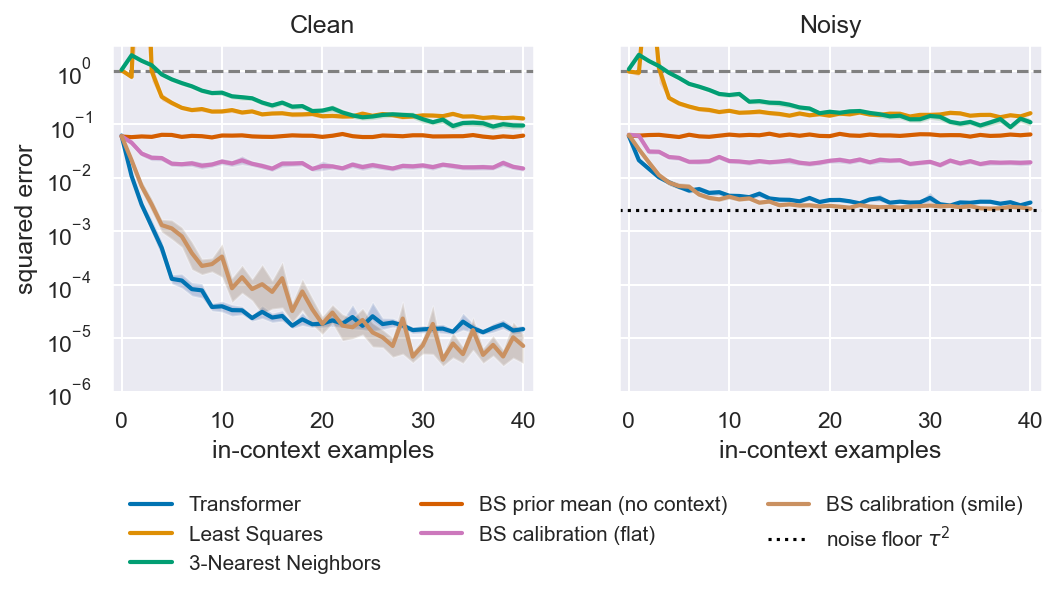
\includegraphics[width=0.9\linewidth]{figures/bs_smile/clean_vs_noisy.png}
\caption{\textbf{[YOUR caption: smile volatility; clean vs.\ noisy; gray dashed line =
error 1; dotted line = noise floor $\tau^2$]}}
\label{fig:bs-smile-noise}
\end{figure}

\paragraph{Scaled moneyness.}
On smile volatility (Figure~\ref{fig:bs-smile-scaling}), scaling by 2 leaves the
transformer's error at $k=40$ at $7.0\cdot10^{-4}$, still far below the prior mean (0.060),
but it stops improving after a few examples. Scaling by 3, it stays around $0.06$ for all
$k$ ($0.063$ at $k=40$), only slightly below the prior mean ($0.100$). Smile calibration
reaches at most $2.3\cdot10^{-6}$ in all cases, while misspecified flat calibration is
worse than the prior mean at scale 3 ($0.28$). On flat volatility the failure is even
clearer: at scale 3 the transformer's error ($0.082$) is above the prior mean ($0.073$) for
all $k$, i.e.\ it does worse than ignoring the examples, while calibration reaches
$6.3\cdot10^{-7}$.
\textbf{[What has the transformer learned, given that it works at $\times 2$ and fails at
$\times 3$? Why is calibration unaffected? Parallel to \cite{garg2022what}?]}

\begin{figure}[h]
\centering
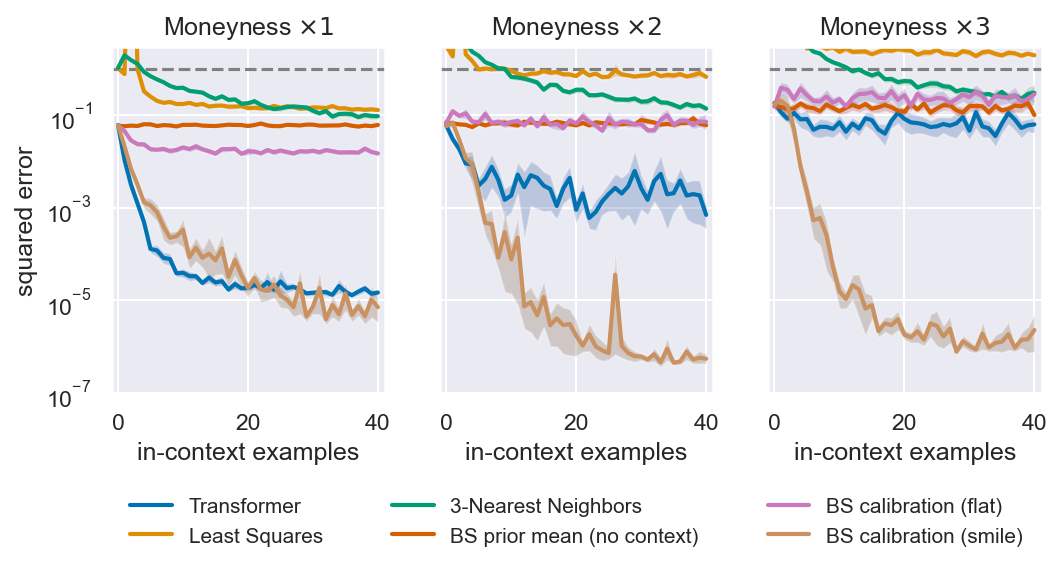
\includegraphics[width=0.9\linewidth]{figures/bs_smile/moneyness_scaling.png}
\caption{\textbf{[YOUR caption: smile volatility; moneyness scaled by 1, 2, 3 at test
time without retraining; gray dashed line = error 1]}}
\label{fig:bs-smile-scaling}
\end{figure}

\paragraph{Discussion and Limitations.}
Finding 1: the transformer falls below the prior mean after one example, and far
below flat calibration on smile volatility. What does each comparison rule out, i.e.\
which ``lazy'' strategy would each have caught?

Finding 2: on smile volatility the transformer beats calibration with the correct
model up to $k \approx 18$. What does the transformer have that calibration lacks, and why
does that advantage disappear at large $k$?

Finding 3: at moneyness $\times 3$ the transformer stops improving, while
calibration is unaffected. What does that say about what the transformer has learned:
the Black--Scholes formula itself, or something else? How does it compare with linear
regression under input scaling in \cite{garg2022what}?

Limitations: finish ``Because of this, we cannot claim that \ldots'' for
(i) one training run per task without a fixed seed;
(ii) no posterior-mean (Bayes-optimal) baseline;
(iii) the pricing formula and $r$ are the same in every prompt.